\documentclass[11pt]{jsarticle}

\usepackage{multirow}
\usepackage{bm}
\usepackage{makeidx}

\usepackage{wrapfig}

\usepackage{amsmath,amsthm,amssymb}
\usepackage[dvipdfmx]{graphicx}

%% 高さの設定
\setlength{\textheight}{\paperheight}   % ひとまず紙面を本文領域に
\setlength{\topmargin}{-5.4truemm}      % 上の余白を20mm(=1inch-5.4mm)に
\addtolength{\topmargin}{-\headheight}  % 
\addtolength{\topmargin}{-\headsep}     % ヘッダの分だけ本文領域を移動させる
\addtolength{\textheight}{-40truemm}    % 下の余白も20mmに%% 幅の設定
\setlength{\textwidth}{\paperwidth}     % ひとまず紙面を本文領域に
\setlength{\oddsidemargin}{-5.4truemm}  % 左の余白を20mm(=1inch-5.4mm)に
\setlength{\evensidemargin}{-5.4truemm} % 
\addtolength{\textwidth}{-40truemm}     % 右の余白も20mmに

%\abovecaptionskip=-2pt
\belowcaptionskip=-10pt

\makeatletter 
\def\section{\@startsection {section}{1}{\z@}{1.5 ex plus 2ex minus -.2ex}{0.5 ex plus .2ex}{\large\bf}}
\def\subsection{\@startsection{subsection}{2}{\z@}{0.2\Cvs \@plus.5\Cdp \@minus.2\Cdp}{0.1\Cvs \@plus.3\Cdp}{\reset@font\normalsize\bfseries}}
\makeatother 

\begin{document}

%%%%%%
% はじめに
%%%%%%
\begin{center}
{\Large \textgt{34. DPD シミュレーションによる動的ネットワークの緩和挙動の検討}}
\end{center}

\begin{flushright}
東亞合成 ${}^\circ$佐々木裕\\
近大理工 荒井規允

Tel: 052-611-9923, e-mail: hiroshi\_sasaki$@$mail.toagosei.co.jp
\end{flushright}

\vspace{0.5\baselineskip}
\section{はじめに}
\subsection{背景}

近年、ソフトマター研究~\cite{DeGennes1992}の深化に伴い、ソフトマターの内部自由度の高さを利用した階層的な構造設計の検討が進んでおり~\cite{Deng2010}、ソフトマターの特徴である柔らかさに加えて各種の新規機能を付加した材料の開発が活発に行われている。
力学的な機能を検討する場合には、系全体の流動を抑制した固体的な特性を要求され、ネットワーク構造が必要となる場合が多い。

ネットワーク構造を有するソフトマターの研究開発の流れに注目すると、旧知の材料であるゴムの機能性の発現機構の解明~\cite{Qu2011}も精力的に行われており、また、脆い材料として知られているゲルについてもこれまでにない高強度なものが発見されてきている~\cite{Ito2007,Gong2010}。%,Zhao2014
これらのネットワークポリマーの材料設計においては、フィラー同士の相互作用のような比較的大きなスケールの構造の寄与も大きい~\cite{Qu2011}が、ネットワーク構造の均一性もマクロな特性に大きな影響を与え、
%るため、架橋構造の形成が重要なポイントとなる。
単純な化学架橋で
%を行った場合には、
形成されるネットワーク構造には空間的な不均一(架橋密度揺らぎ)が生じてしまうことが知られている。
酒井らは、溶液中でのポリマー濃度を調整することで、均質なネットワーク構造を有するゲル(tetra-PEG gel)を形成できることを報告している~\cite{Sakai2008}。


一方、無溶剤での構造の明確なネットワークの形成としては、水素結合、疎水性相互作用、静電相互作用などの「繋ぎ替え可能な非共有結合」を介して自己組織化した超分子ネットワークも報告されてきている~\cite{Sijbesma1997,CHINO2005}。

% \begin{wrapfigure}{r}{50mm}
% %\vspace{-1\baselineskip}
% %	\begin{center}
% 		\begin{table}[htb]
%  		\caption{aa}
%  		\centering
%  		\begin{tabular}{|c|c|} \hline
% 		a & c \\ \hline \hline
% 		b & d \\ \hline
%  		\end{tabular}
%  		\label{tbl: •}
% 		\end{table}
% %		\label{fig: TouchPanel}
% %		\caption{スマートフォン等のタッチパネル搭載機器での粘着剤}
% %	\end{center}
% %\vspace{-1\baselineskip}
% \end{wrapfigure}

\subsection{本日の発表内容}
本日の発表では、オリゴマーの特性を利用した材料設計の例として、スマートフォン等でなじみの深い「タッチパネル粘接着剤」の改質を検討した例を題材として話題提供を行う。
まず、「高温ラジカル重合によるオリゴマー製造」についての簡単な紹介を行った後、「タッチパネル粘接着剤用オリゴマーの開発」について、要求特性を充足するために行った各種の評価方法等の説明を行う。
さらに、良好な特性を示すオリゴマー添加剤の機能発現メカニズムについても解析を行っているので、その内容も解説する予定である。

\section{シミュレーション}

本研究では散逸粒子動力学(DPD)法を使用した~\cite{Groot1997}。
DPD法では複数の粒子を一つの粒子として粗視化して扱い、各粒子間に働く力は下式で与えられる。
\begin{equation}
m\dfrac{{\rm d}^2 {\bf r}_i}{{\rm d} t^2} = {\bf f}_i = \sum_{j \neq i} \left( {\bf F}_{ij}^C + {\bf F}_{ij}^D + {\bf F}_{ij}^R \right)
\end{equation}
ここで、${\bf F}_{ij}^C, {\bf F}_{ij}^D, {\bf F}_{ij}^R$ はそれぞれ $i$ 粒子と $j$ 粒子の間に働く保存力、 散逸力、ランダム力を表す。

$\mathbf{F}_{ij}^C$ は、粒子 $i$ と $j$ との間に働く通常の粒子間相互作用であり、粒子間の相対位置ベクトル$\mathbf{r}_{ij} (=\mathbf{r}_i - \mathbf{r}_j)$ にのみ依存し、速度には依存しないと仮定でき、以下のように書ける。
\begin{equation}
	\mathbf{F}_{ij}^C =
        \begin{cases}
        	a_{ij} w^C (|\mathbf{r}_{ij}|) \dfrac{\mathbf{r}_{ij}}{|\mathbf{r}_{ij}|} & (|\mathbf{r}_{ij}| < r_c) \\
                0 & (|\mathbf{r}_{ij}| \geq r_c)
        \end{cases}
\end{equation}
ここで、$a_{ij}$ は粒子間の斥力の大きさを表す係数、$w^C (|\mathbf{r}_{ij}|)$ は粒子間距離に応じてそれらの間に作用する力を減少させるための重み関数であり、また、 r$_c$ はカットオフ距離を表し、これより遠い距離の相互作用は無視されることになる。


\begin{equation}
\dfrac{\chi N k_B T}{\Delta a} = \left( 0.3003 \pm 0.003 \right)N
\end{equation}

\begin{equation}
\dfrac{\chi N k_B T}{\Delta a} = (0.306 \pm 0.003) N
\end{equation}

テレケリックポリマーの計算モデルとして、20個のビーズから成るA1B18A1トリブロックポリマーを使用し、トリブロックポリマーの末端が作るクラスターからの引き抜きを観察した。
計算条件はA1B18A1トリブロックポリマー1200本、総ビーズ数は24,000個、密度 $\rho =3$ とした。

保存力に含まれる相互作用パラメータ $a_ij$ によって、ビーズ間に働く斥力の大きさが決定される。
同種ビーズ間に比べ、異種間のビーズに対し、ある程度大きな斥力(約3倍)を設定したところ、適度な大きさのクラスターが得られた。

\section{結果と考察}

ああああああああああああああああああああああああああああああ

ああああああああああああああああああああああああああああ

\begin{wrapfigure}{r}{100mm}
\vspace{-1\baselineskip}
	\begin{center}
		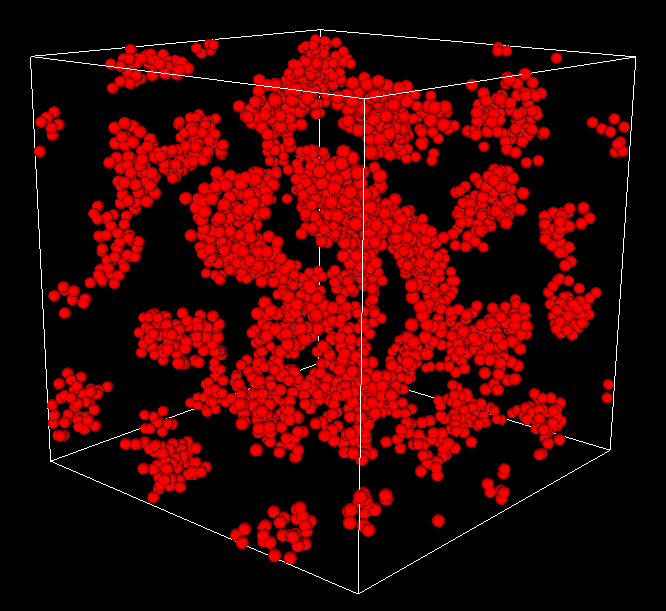
\includegraphics[width=100mm]{./fig/Snap.png}
		\label{fig: TouchPanel}
		\caption{スマートフォン等のタッチパネル搭載機器での粘着剤}
	\end{center}
\vspace{-1\baselineskip}
\end{wrapfigure}

\section{おわりに}

本日のメインテーマである「高分子反応の新展開」からは、いささか逸脱した話題となってしまったが、高分子特有の性質を利用した材料設計の一例として、「タッチパネル粘接着剤用オリゴマーの開発」についての紹介を行った。

今回対象とした材料は、弊社で以前より開発を行ってきた「高温ラジカル重合によるオリゴマー」を対象としたものであり、この特性を生かせるような用途として開発ターゲットを選定している。
材料としてみた場合に粘接着剤の主役は高分子量のポリマーであるが、そこに分子量の大きく異なるオリゴマーを配合することによりバルクでの材料特性を大きく改良することができることが確認できた。

今回の事例では反応性を付与したものを使用してはいないが、反応性を付与したオリゴマーにおいても同様の振る舞いは期待できる。
高分子特有の振る舞いを利用することにより、ミクロでローカルな界面の物性を制御することで接着性等のマクロな物性を改良し、接着という機能をさらに高められるものと期待している。

\bibliographystyle{achemso}
%{elsart-num}
%{junsrt-2}
\bibliography{D:/Dropbox/Tex/Bibliography/library.bib}

\end{document}